\section{应用前景:分布式成像}
\subsection{分布式成像仿真结果对比}
针对于前文的成像需要一个大的接收机阵列以及较大的两路接收机间距以消除频偏等问题,利用分布式
成像的方式是一个可能的潜在应用场景。这里给出了一个分布式成像的例子,如图~\ref{分布式成像仿真场景}所示。
需要注意的是,这里对$N=96$的接收阵列成像情形以及三个$N=32$的接收阵列分布式成像的结果进行了对比,并且
这里的成像结果考虑了对信源(发射机)的成像。
\begin{figure}[H]
  \centering
  \begin{subfigure}[t]{.45\linewidth}
    \centering
    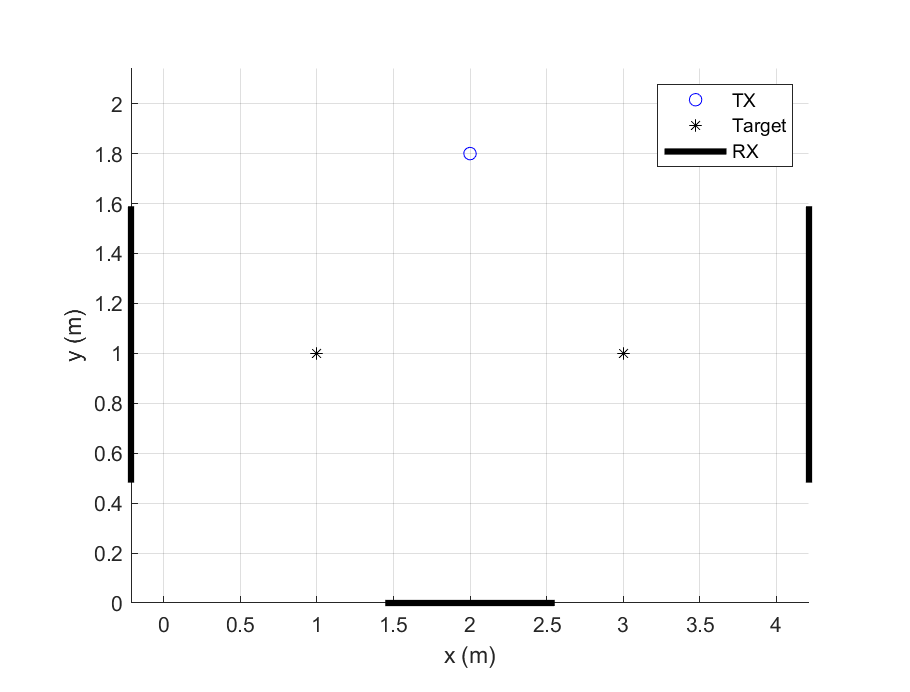
\includegraphics[width=1\textwidth]{figures/distribution/model1_circ.eps}
    \caption{$3$个$N=32$接收机阵列分布式成像}  
  \end{subfigure}
  \begin{subfigure}[t]{.45\linewidth}
    \centering
    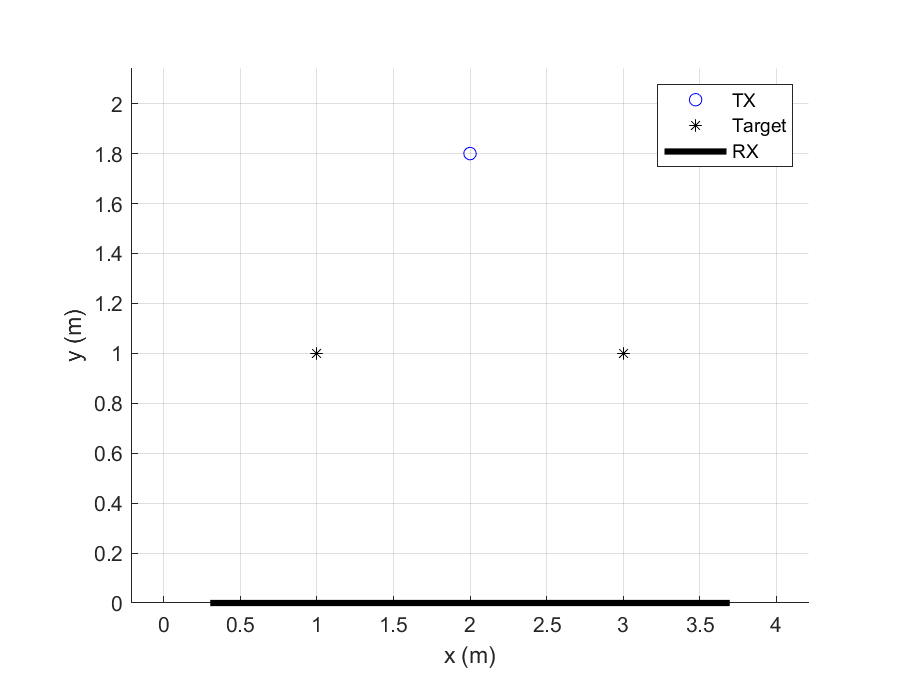
\includegraphics[width=1\textwidth]{figures/distribution/model1.eps}
    \caption{对比:单个$N=96$接收机阵列成像}
  \end{subfigure}
  \caption{分布式成像仿真场景}
  \label{分布式成像仿真场景}
\end{figure}
分布式成像添加的频偏与单阵列成像添加的频偏一致(服从公式~\eqref{情形二}),具体的仿真参数见表~\ref{分布式成像仿真设置},
仿真结果如图~\ref{分布式成像仿真结果}所示,可以看出,在理想成像或频偏影响较小的情况下,分布式成像具有和单阵列成像相近或更好的效果。
\begin{table}[htb]
  % h-here,t-top,b-bottom,优先级依次下降
      \begin{center}
      % 居中
          \caption{分布式成像仿真设置}\label{分布式成像仿真设置}
          \begin{tabular}{lc} % 三线表不能有竖线,l-left,c-center,r-right
              \toprule
              %三线表-top 线
              参数 & 值 \\
              \midrule
              %三线表-middle 线
              是否考虑对信源(发射机)成像 & 是(仿真多径设置了LOS径)\\
              是否考虑CSI频偏的影响 & 是\\
              考虑频偏的情形  & 服从公式~\eqref{情形二}\\
              采样频率偏移(SFO)   &   $\theta_{\text{sfo}}\sim N(0,100)$ Hz\\
              包检测误差(PDP)     &   $\theta_{\text{pdd}}\sim N(0,100)$ Hz\\
              载波频率偏移(CFO)   &   $\theta_{\text{cfo}}\sim N(0,1000)$ Hz\\
              成像目标数量(含信源)    & 3\\
              信源位置        &  $(2\text{米},1.8\text{米})$ \\
              成像目标的位置  & $(1\text{米},1\text{米})$,$(3\text{米},1\text{米})$ \\
              工作频点        & $4.2$GHz\\
              工作带宽      & 20MHz \\
              子载波数目      & 256\\
              发射机位置           & $(2\text{米},0\text{米})$\\
              接收机天线阵元数$N$      & $3*32$\\
              接收机天线阵元间隔    & 半波长(约$3.57$厘米)\\
              接收机位置           & 如图~\ref{分布式成像仿真场景}\\
              两路接收天线的位置差$\Delta_d$ & $1$米\\
              \bottomrule
              %三线表-底线
          \end{tabular}
      \end{center}
\end{table}

\begin{figure}[H]
  \centering
  \begin{subfigure}[t]{.3\linewidth}
    \centering
    \includegraphics[width=1\textwidth]{figures/distribution/expected/array.eps}
    \caption{未添加频偏~单阵列成像}
  \end{subfigure}
  \begin{subfigure}[t]{.3\linewidth}
    \centering
    \includegraphics[width=1\textwidth]{figures/distribution/expected/joint.eps}
    \caption{未添加频偏~三个分布式阵列合并为单阵列}
  \end{subfigure}
  \begin{subfigure}[t]{.3\linewidth}
    \centering
    \includegraphics[width=1\textwidth]{figures/distribution/expected/multiplication.eps}
    \caption{未添加频偏~三个分布式阵列分别成像再相乘}
  \end{subfigure}
  \\
  \begin{subfigure}[t]{.3\linewidth}
    \centering
    \includegraphics[width=1\textwidth]{figures/distribution/freq/array.eps}
    \caption{情形二频偏~单阵列成像}
  \end{subfigure}
  \begin{subfigure}[t]{.3\linewidth}
    \centering
    \includegraphics[width=1\textwidth]{figures/distribution/freq/joint.eps}
    \caption{情形二频偏~三个分布式阵列合并为单阵列}
  \end{subfigure}
  \begin{subfigure}[t]{.3\linewidth}
    \centering
    \includegraphics[width=1\textwidth]{figures/distribution/freq/multiplication.eps}
    \caption{情形二频偏~三个分布式阵列分别成像再相乘}
  \end{subfigure}
  \caption{分布式成像仿真结果}\label{分布式成像仿真结果}
\end{figure}

\begin{figure}[htb]
  \centering
  \begin{subfigure}[t]{.45\linewidth}
    \centering
    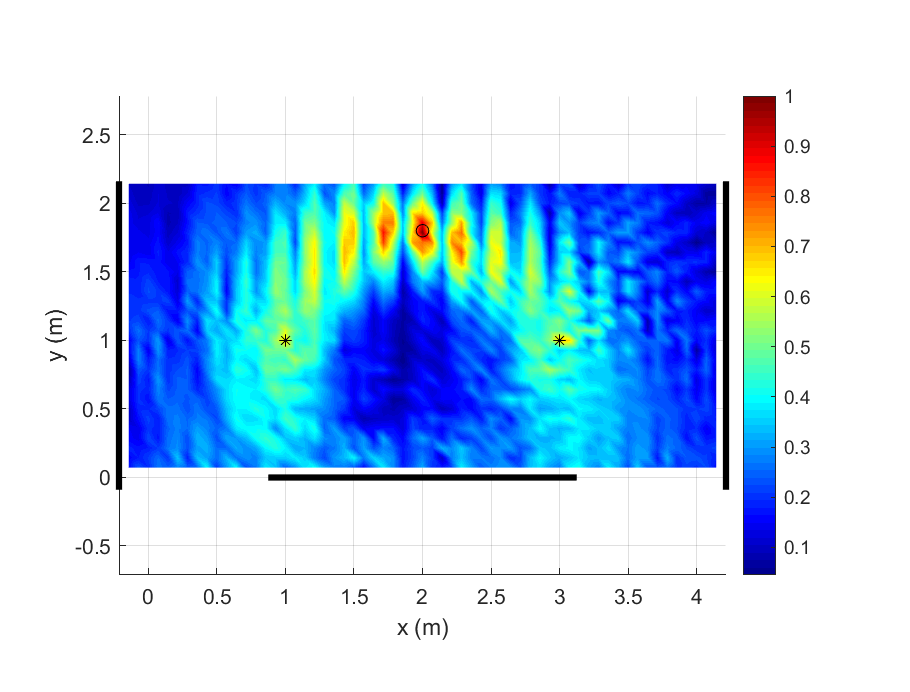
\includegraphics[width=\textwidth]{figures/distribution/TPF/1.eps}
    \caption{无频偏~每个子阵列分别加汉明窗}
  \end{subfigure}
  \begin{subfigure}[t]{.45\linewidth}
    \centering
    \includegraphics[width=\textwidth]{figures/distribution/TPF/2.eps}
    \caption{情形二频偏~每个子阵列分别加汉明窗}
  \end{subfigure}
  \begin{subfigure}[t]{.45\linewidth}
    \centering
    \includegraphics[width=\textwidth]{figures/distribution/TPF/3.eps}
    \caption{无频偏~子阵列串联后整体加窗}
  \end{subfigure}
  \begin{subfigure}[t]{.45\linewidth}
    \centering
    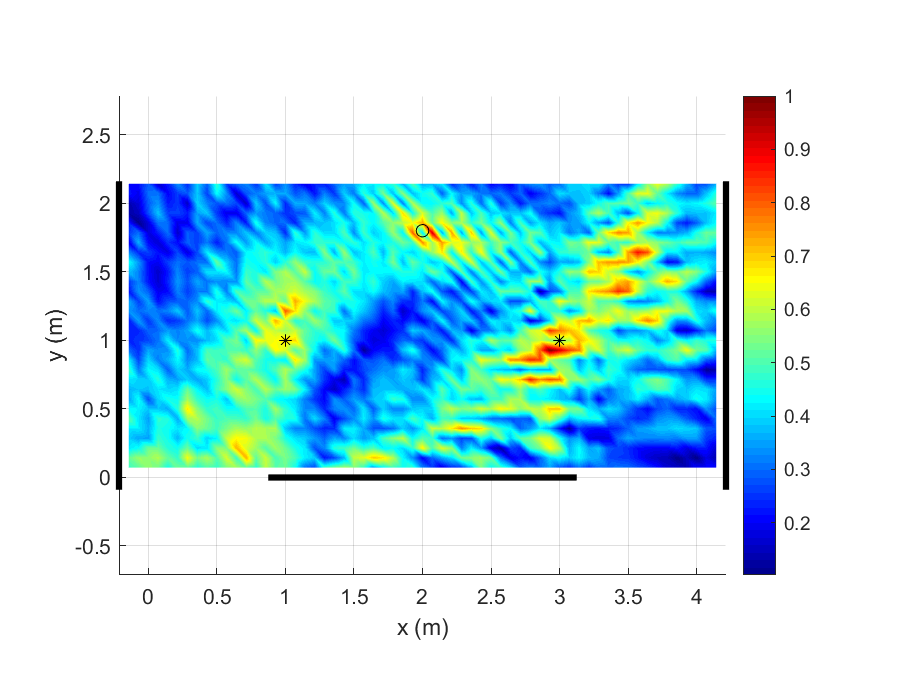
\includegraphics[width=\textwidth]{figures/distribution/TPF/4.eps}
    \caption{情形二频偏~子阵列串联后整体加窗}
  \end{subfigure}
  \caption{结合PARAFAC算法的分布式成像仿真结果}
  \label{TPF分布式}
\end{figure}

\subsection{结合PARAFAC算法的分布式成像仿真结果}
结合PARAFAC算法与共轭相乘消除频偏的仿真采取$N=3*64$,$\delta_d=0.8$米的接收天线阵列,其余参数与表~\ref{分布式成像仿真设置}一致。
仿真结果如图~\ref{TPF分布式}所示,需要注意的是,这里我们还尝试了子阵列成像结果分别汉明窗以及子阵列联合成像结果加统一的汉明窗对结果的影响,
可以看出,子阵列分别加汉明窗具有更好的成像效果。